\documentclass[xcolor=pdftex,dvipsnames,table,mathserif,aspectratio=169]{beamer}
\usetheme{metropolis}
%\usetheme{Darmstadt}
%\usepackage{times}
%\usefonttheme{structurebold}

\usepackage[english]{babel}
%\usepackage[table]{xcolor}
\usepackage{pgf,pgfarrows,pgfnodes,pgfautomata,pgfheaps}
\usepackage{amsmath,amssymb,setspace}
\usepackage[latin1]{inputenc}
\usepackage[T1]{fontenc}
\usepackage{relsize}
\usepackage[absolute,overlay]{textpos} 
\newenvironment{reference}[2]{% 
  \begin{textblock*}{\textwidth}(#1,#2) 
      \footnotesize\it\bgroup\color{red!50!black}}{\egroup\end{textblock*}} 

\DeclareMathSizes{10}{10}{6}{6} 


\title [Dynamic Oligopoly I]{Switching Costs: Orange Juice}
\author{C.Conlon }
\institute{Grad IO }
\date{Fall 2020}
\setbeamerfont{equation}{size=\tiny}
\begin{document}

\begin{frame}
\titlepage
\end{frame}


\begin{frame}{Additional Reading}
You may want to take at the handbook chapter of Farrel and Klemperer for a review of the (largely theoretical) literature.

\end{frame}
\begin{frame}{State Dependence}
Think about a static model like BLP
\begin{eqnarray*}
u_{ijt} = \beta_i x_{jt} - \alpha_i p_{jt} + \xi_{jt} + \varepsilon_{ijt}
\end{eqnarray*}
\begin{itemize}
\item Suppose I have panel data on consumer $i$'s purchases and I observe that the consumer chooses different brands over time
\item Why do you switch brands?  $\beta_i$ are persistent.
\begin{enumerate}
\item New $\varepsilon \rightarrow$ not helpful!
\item Price responses $\rightarrow$ may wrongly attribute all effects to price.
\item $\xi_{jt}$ not correlated across individuals but may include things like advertising, etc.
\end{enumerate}
\item Challenge is explaining both \alert{persistence} and \alert{switching} behavior.
\end{itemize}
\end{frame} 



\begin{frame}{Terminology}
Sometimes we call these models \alert{switching costs} and other times \alert{state dependence}
\begin{eqnarray*}
u_{ijt} = \beta_i x_{jt} - \alpha_i p_{jt} + \xi_{jt} + \alert{\gamma_i \cdot I[y_{i,t-1}=j]} + \varepsilon_{ijt} 
\end{eqnarray*}
\begin{itemize}
\item The idea is purchases in period $t-1$ have a causal effect on utility in period $t$
\item We can think of this as either increasing utility for $j$ if you previously purchased it or providing an additional cost if $y_{it} \neq y_{i,t-1}$.
\end{itemize}
\end{frame} 


\begin{frame}{Why Do We Care?}
\begin{itemize}
\item Switching costs appear to be a real friction in the economy.
\item Consumers are often highly persistent in product choices.
\begin{itemize}
\item Because they really like the product?
\item Because they are unaware of alternatives?
\item Because they are lazy?
\end{itemize}
\item Extremely important in the market for \alert{health insurance}. Consumers in ACA (Obamacare) exchanges would have saved \$610/yr on average if they switched to a lower cost plan in the same tier.
\begin{itemize}
\item Real costs associated with switching: checking to see if my doctor takes the other insurer, calculating expected expenditures, etc.
\end{itemize}
\item Can we reduce or exploit frictions with laws? defaults? etc.
\end{itemize}
\end{frame} 

\begin{frame}{Why Do We Care?}
\begin{itemize}
\item Switching costs are another way to escape the Bertrand trap for firms which sell relatively undifferentiated products.
\item Old idea going back to Klemperer (1995), Farrell and Klemperer (2007). Do switching costs make markets more or less competitive?
\item Two incentives:
\begin{itemize}
\item \alert{Investment}: Sign up a bunch of consumers today and they will be ``sticky'' to you in the future $\rightarrow$ \alert{lower prices}
\item \alert{Harvesting}: You have additional market power over your ``sticky'' customers $\rightarrow$ \alert{higher prices}
\end{itemize}
\item Most people believe that \alert{harvesting} dominates, and switching costs lead to \alert{higher} prices. (But not always...)
\end{itemize}
\end{frame} 

\begin{frame}{Cabral (JMR 2008)}
Consider dynamic optimization problem faced by firm $i$ with a vector of prices $\mathbf{p}$ and state variables (shares) $\mathbf{x}$ and switching costs $s$:
\begin{eqnarray*}
V_i(\mathbf{x},\mathbf{p},s) = (p_i - c_i) \cdot q_i(\mathbf{x},\mathbf{p},s) + \beta \tilde{V}_i(\mathbf{x},\mathbf{p},s)
\end{eqnarray*}
with FOC
\vspace{-.3cm}
\begin{eqnarray*}
q_i(\mathbf{x},\mathbf{p},s) +  (p_i - c_i) \cdot \underbrace{\frac{\partial q_i(\mathbf{x},\mathbf{p},s)}{\partial p_i}}_{q_i'} +  \beta  \underbrace{\frac{\partial \tilde{V}_i(\mathbf{x},\mathbf{p},s)}{\partial p_i}}_{\tilde{V}_i' \frac{\partial q_i}{\partial p_i}}
\end{eqnarray*}
\vspace{-.3cm}
Define $\tilde{V}_i' \equiv \frac{\partial \tilde{V}_i}{\partial q_i}$ (note w.r.t. $q_i$ not $p_i$). So that:
\begin{eqnarray*}
p_i - c_i = \underbrace{\frac{q_i}{-q_i'}}_{\alert{\mbox{Harvesting}}} - \underbrace{\beta \tilde{V}_i'}_{\alert{\mbox{Investment}}}
\end{eqnarray*}
\end{frame} 

\begin{frame}{Cabral (JMR 2008)}
\small
\begin{eqnarray*}
p_i - c_i = \underbrace{\frac{q_i}{-q_i'}}_{\alert{\mbox{Harvesting}}} - \underbrace{\beta \tilde{V}_i'}_{\alert{\mbox{Investment}}}
\end{eqnarray*}
\vspace{-.3cm}
\begin{itemize}
\item Second term (dynamic benefit of increasing $q_i$ today) is ``investing'' in marketshare and leads to lower PCM.
\item First term is additional market power from switching costs and leads to higher PCM.
\item Take derivatives w.r.t. $s$.
\begin{itemize}
\item It is clear that $|q_i'|$ is decreasing in $s$. Higher switching costs increase static market power.
\item $q_i$ is ambiguous across firms. (So net effect is ambiguous across $i$).
\item $V_i'$ should be zero if $s=0$. And $V_i'$ is increasing in $s$. (Always positive).
\end{itemize}
\item Harvesting can be $\pm$, Investment always $-$.
\end{itemize}
\end{frame} 


\begin{frame}{How do we model these?}
\begin{eqnarray*}
u_{ijt} = \beta_i x_{jt} - \alpha_i p_{jt} + \xi_{jt} + \alert{\gamma_i \cdot I[y_{i,t-1}=j]} + \varepsilon_{ijt} 
\end{eqnarray*}
\begin{itemize}
\item We can include \alert{lagged choice} in utility of the agent. (First order Markov)
\item Could include two lagged choices if we wanted to.
\item Consumers are \alert{not} forward looking. Models are often \alert{time inconsistent}. Why?
\item Has some problems: endogeneity, correlation in $\epsilon_{ijt}$ over time, etc.
\item Fundamental question: How do we identify separately from persistent brand preference?
\item Dube, Histch, Rossi approach: Throw a ton of heterogeneity at the problem.
\end{itemize}
\end{frame} 

\begin{frame}{Mixture of Normals}
Let $\theta_i =[\alpha_i,\beta_i,\gamma_i]$.
\begin{itemize}
\item For each individual draw a class $k$ from a multinomial distribution $\pi$.
\item Now draw $\theta_i \sim MVN(\mu_k, \Sigma_k)$.
\item Idea is that $P(\theta_i | \pi,\mu,\Sigma) = \sum_k \pi_k \phi(\theta_i | \mu_k, \Sigma_k)$ is a mixture of normals. \pause
\item These models are highly flexible (around 4-5 normals tends to well approximate most distributions).
\item But hard to estimate! (Problem is highly non-convex, EM algorithm is slow).
\item In order to do MCMC estimation we have to assume some hyper-parameters $b$ so that we can put a prior on $\pi$ as well as $\mu_k,\Sigma_k$.
\end{itemize}
\end{frame} 



\begin{frame}{Switching Costs in Orange Juice}
\begin{center}
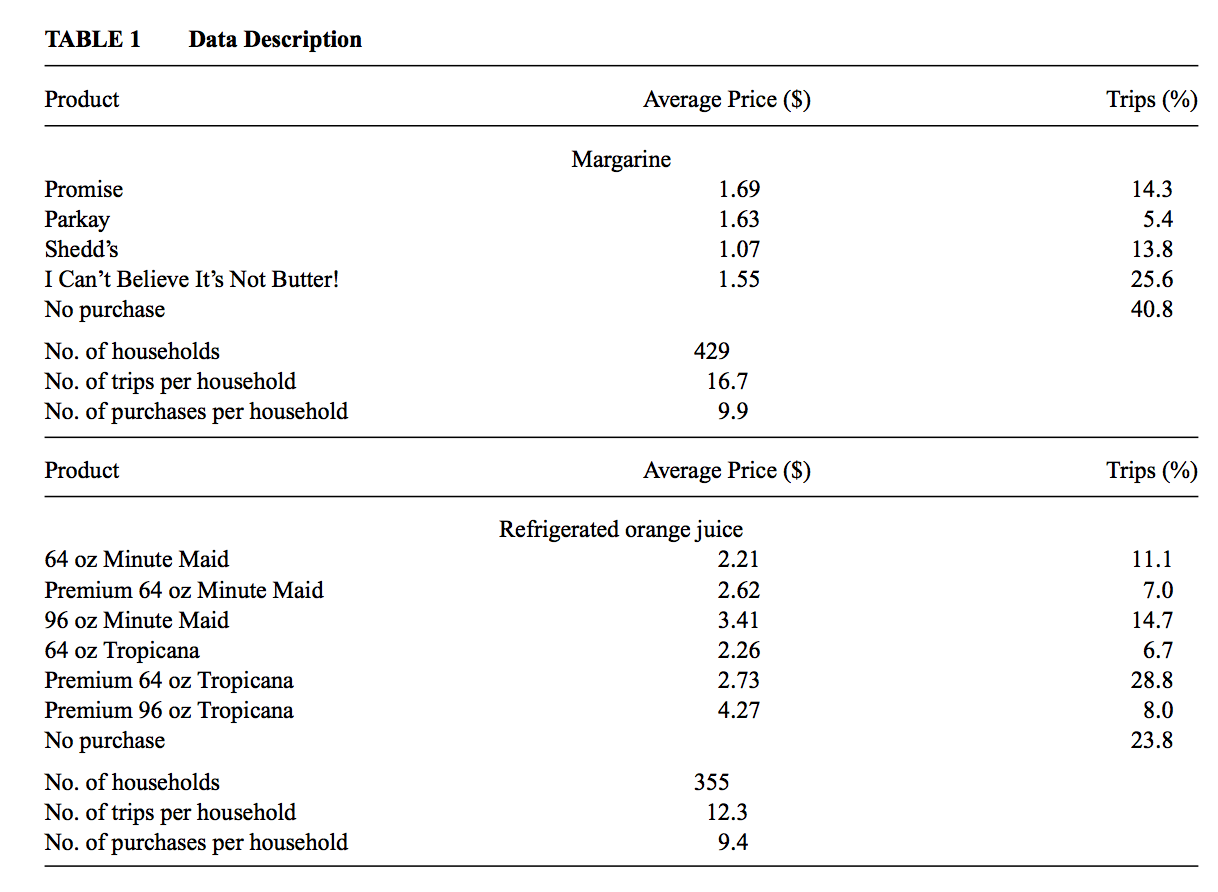
\includegraphics[scale=0.5]{resources/oj_t1.png}
\end{center}
\end{frame}

\begin{frame}{Switching Costs in Orange Juice}
\begin{center}
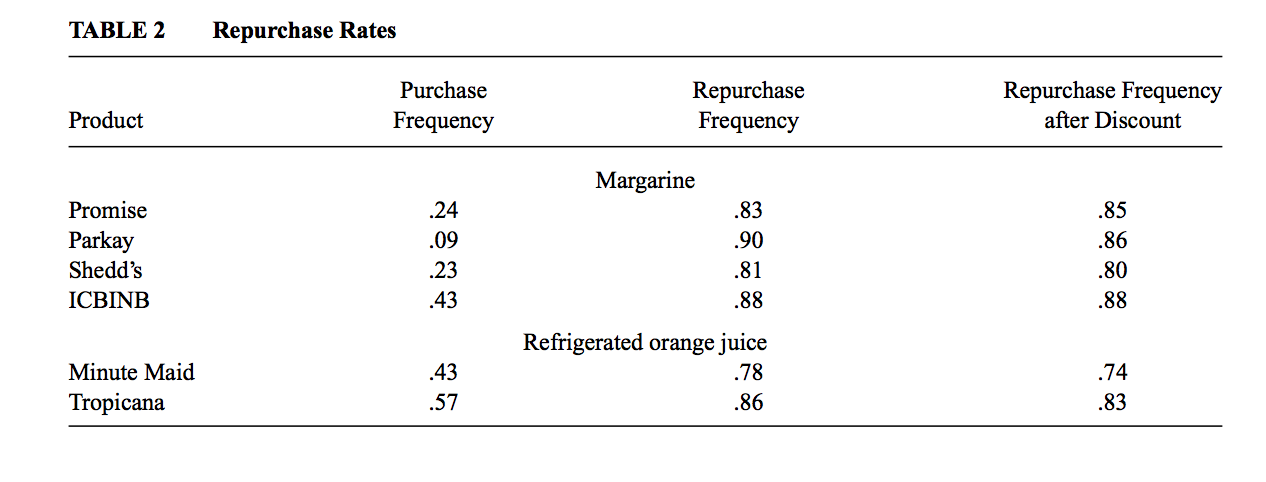
\includegraphics[scale=0.5]{resources/oj_t2.png}
\end{center}
\end{frame}

\begin{frame}{Switching Costs in Orange Juice}
\begin{center}
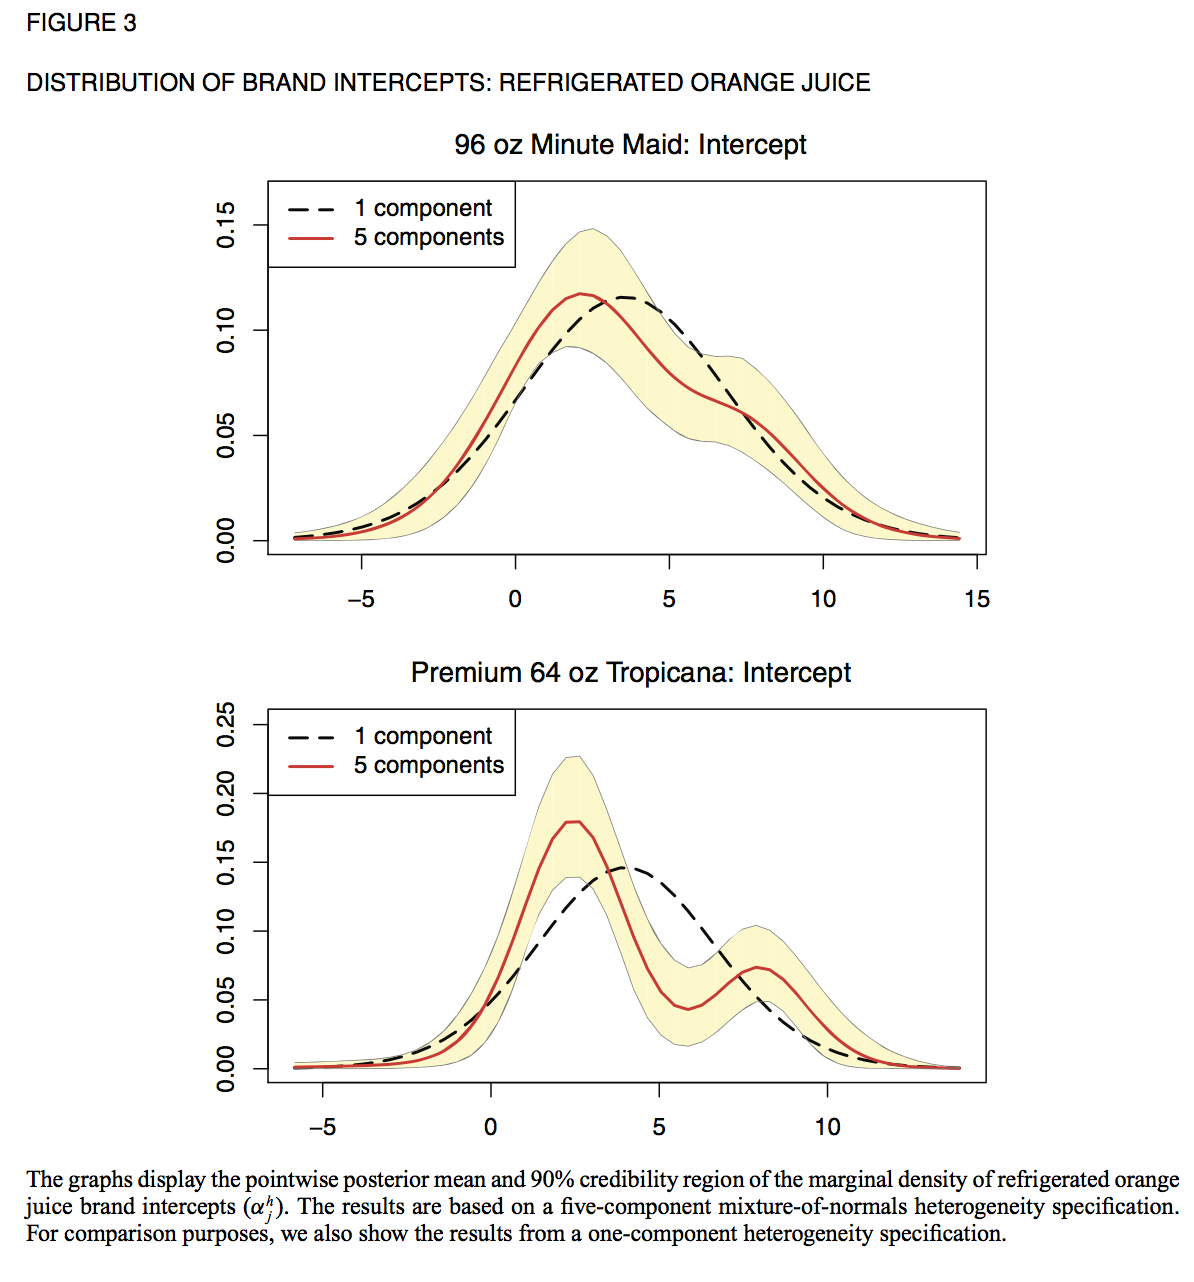
\includegraphics[scale=0.33]{resources/OJ_F3.png}
\end{center}
\end{frame}

\begin{frame}{Switching Costs in Orange Juice}
\begin{center}
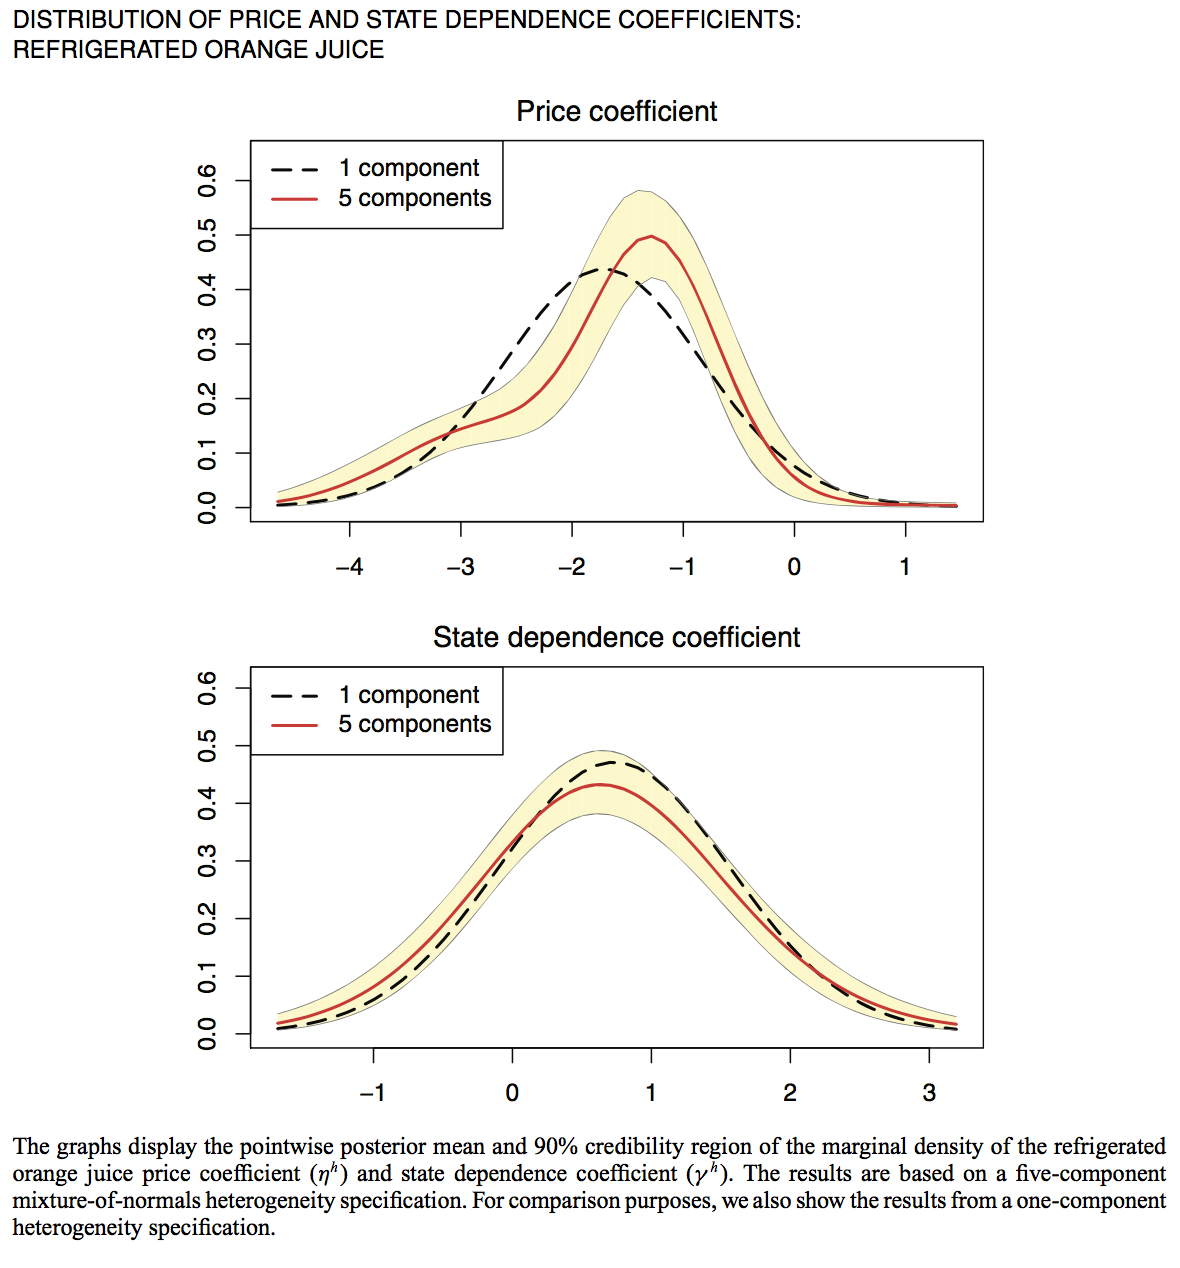
\includegraphics[scale=0.33]{resources/OJ_F4.png}
\end{center}
they also try 10 components...
\end{frame}

\begin{frame}{Identification}
\begin{itemize}
\item Lots of price changes in the category. Imagine two brands $(P,C)$ and each one can set two prices $\{H,L\}$.
\item We observe the sequence $D_1(H,H) = C, D_2(H,L) = C, D_3(H,H) = C, D_4(L,H) = P$.
\item If we see that $D_5(H,H/L) = P$ then we find evidence of state dependence.
\item Likewise we can see you switch, become sticky, and switch back later.
\end{itemize}
\end{frame} 

\begin{frame}{Identification/Robustness}
\begin{itemize}
\item The authors re-arrange the order of purchases within an individual and re-estimate.
\item If this was persistent heterogeneity they should still spuriously find a large $\gamma$
\item They do not!
\end{itemize}
\end{frame}
 
\begin{frame}{Switching Costs in Orange Juice}
\begin{center}
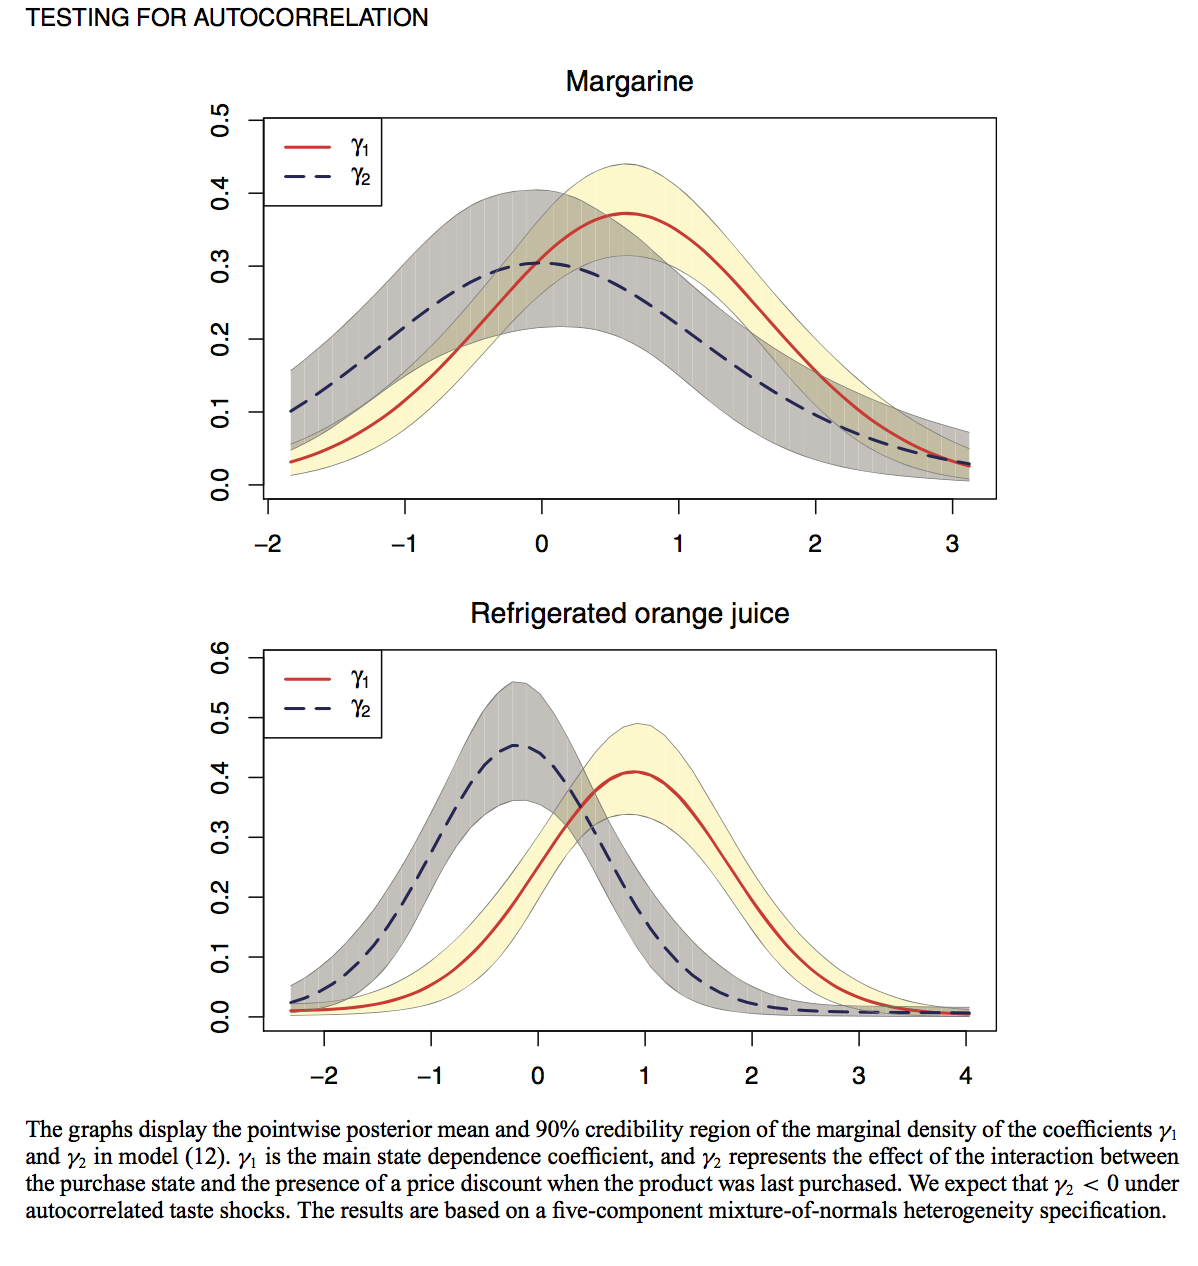
\includegraphics[scale=0.33]{resources/OJ_F5.png}
\end{center}
\end{frame}


\begin{frame}{Switching Costs in Orange Juice}
\begin{center}
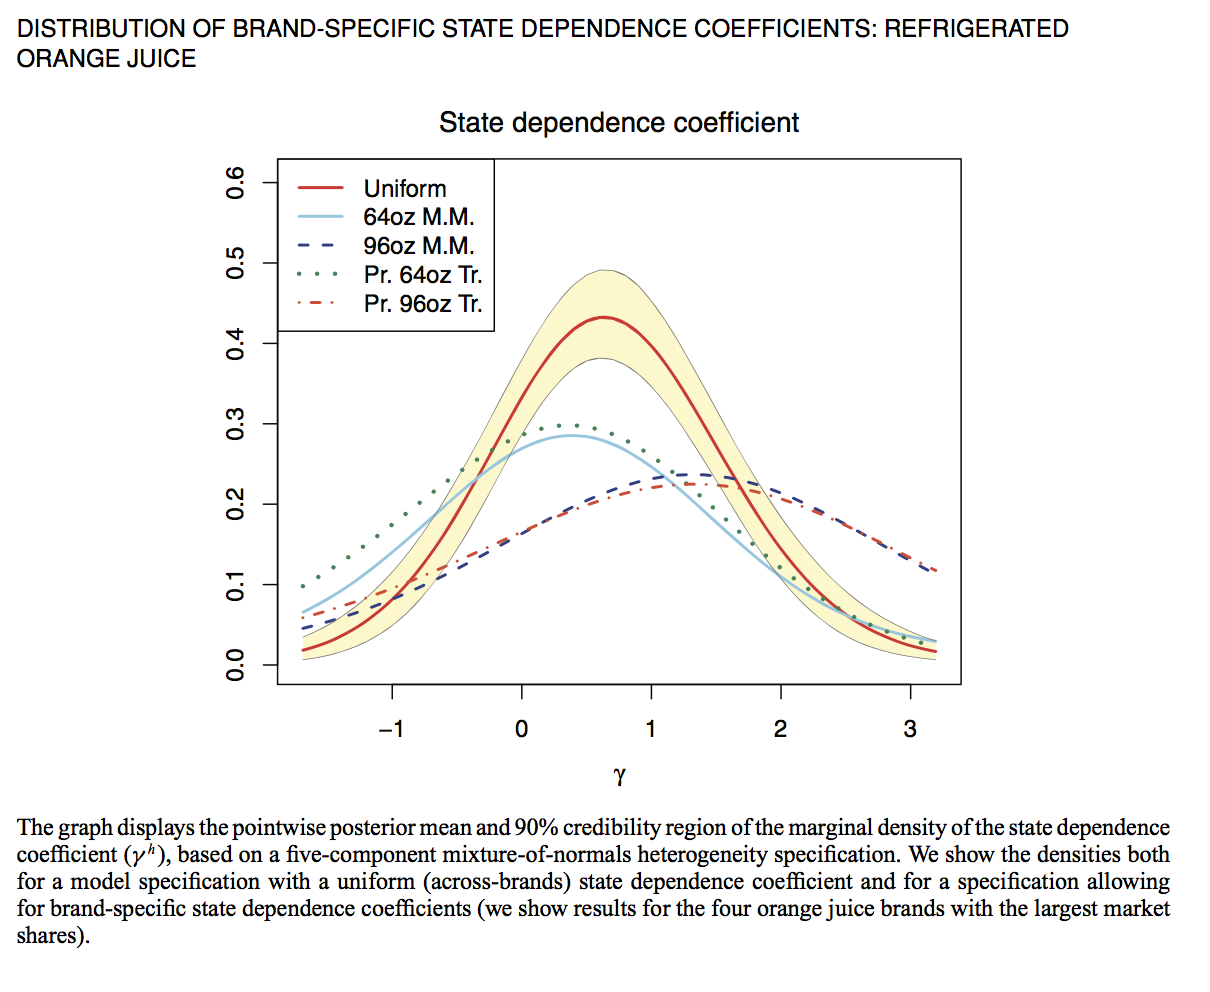
\includegraphics[scale=0.33]{resources/OJ_F8.png}
\end{center}
\end{frame}


\begin{frame}{Switching Costs in Orange Juice}
\begin{center}
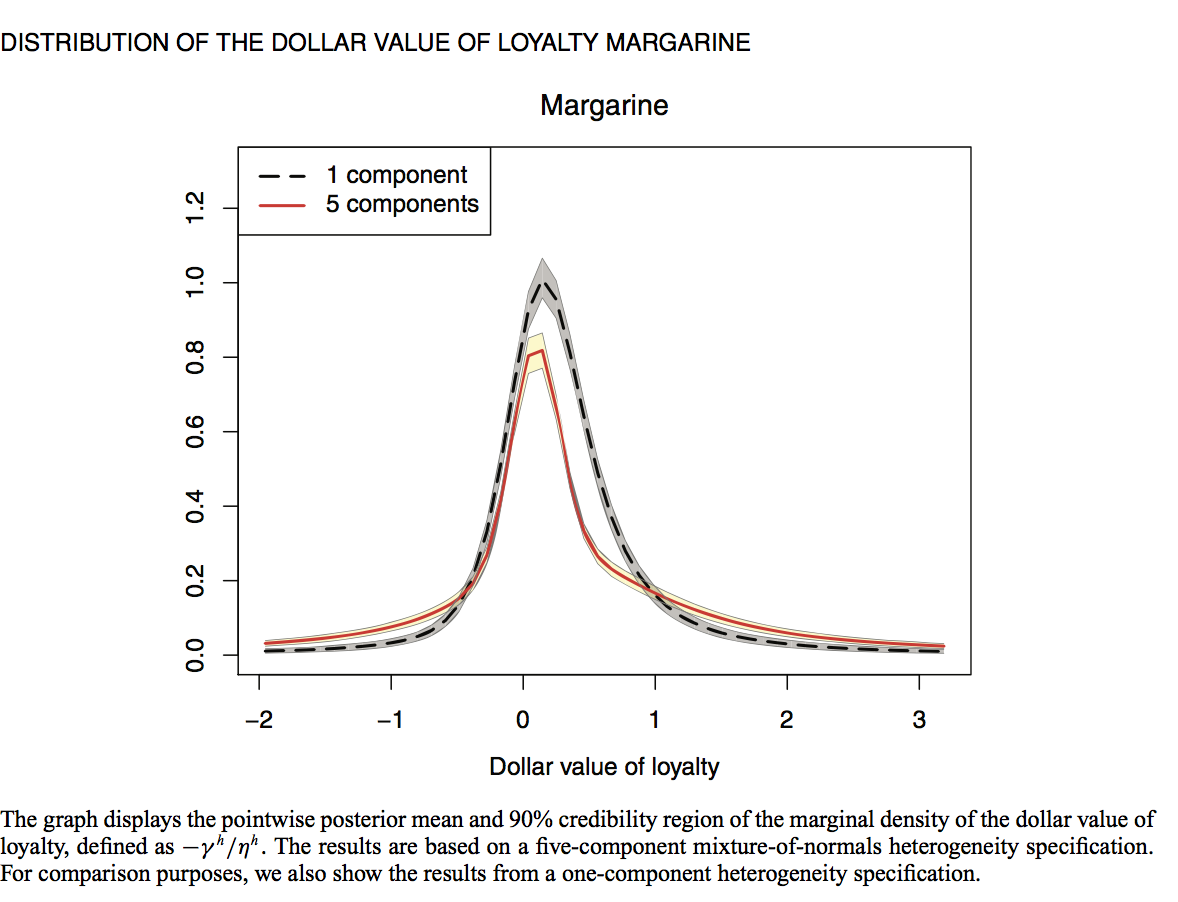
\includegraphics[scale=0.33]{resources/OJ_F11.png}
\end{center}
\end{frame}

\begin{frame}{Why Does this matter}
\begin{itemize}
\item Solve a dynamic programming problem like in Cabral (2008).
\item If we have just auto-correlation and no switching costs, there is NO harvesting incentive.
\item If we have switching costs than there is.
\item Very small switching costs can make markets MORE competitive.
\end{itemize}

\end{frame}


\begin{frame}{Switching Costs in Orange Juice}
\begin{center}
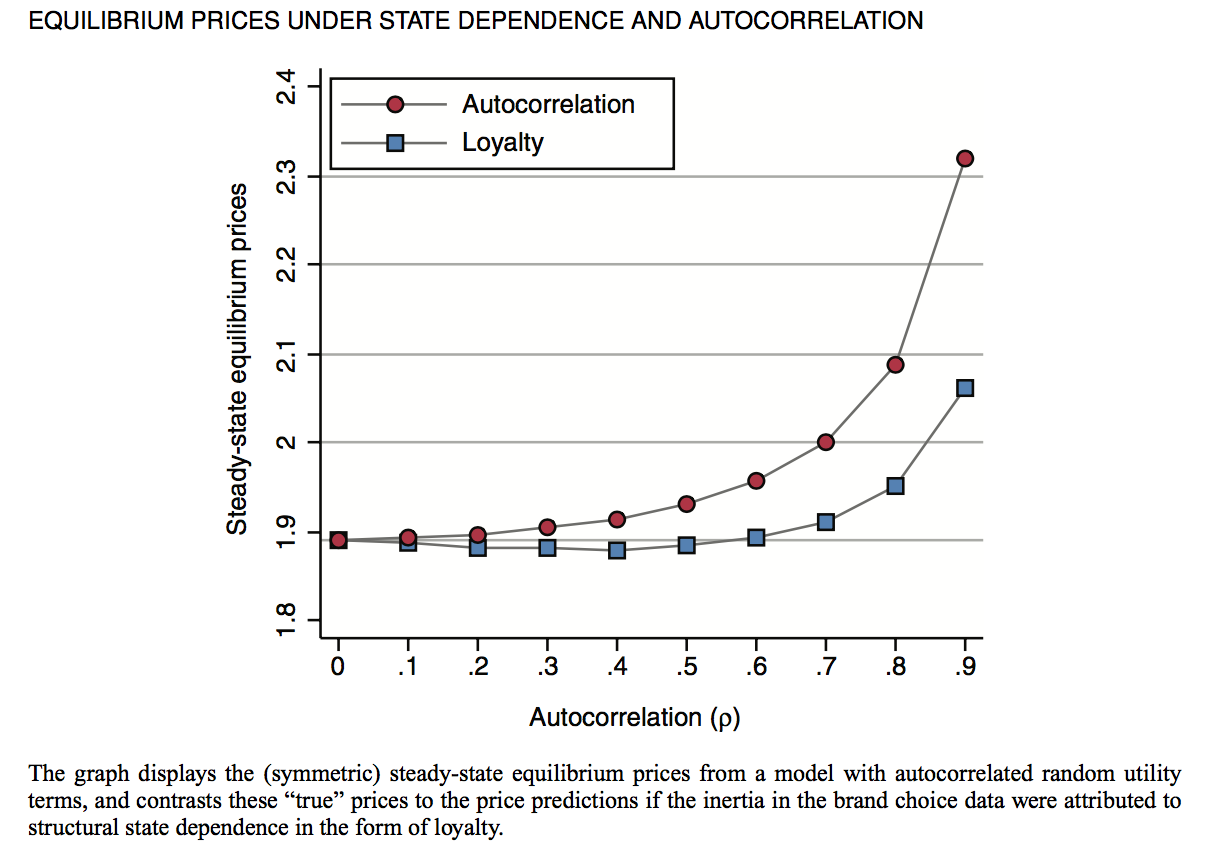
\includegraphics[scale=0.33]{resources/OJ_F12.png}
\end{center}
\end{frame}


\end{document}













































